\section{La Rete Neurale Biologica}
Il miglior modo per capire il funzionamento di una rete neurale è capire come 
funziona un neurone biologico. In quanto le reti neurali artificiali traggono 
ispirazione dal funzionamento dei neuroni che compongono il cervello umano 
\cite{PARAGONE_CERVELLE_RETE_NEURALE_1, PARAGONE_CERVELLE_RETE_NEURALE_2}.

\begin{figure}[h]
    \centering
    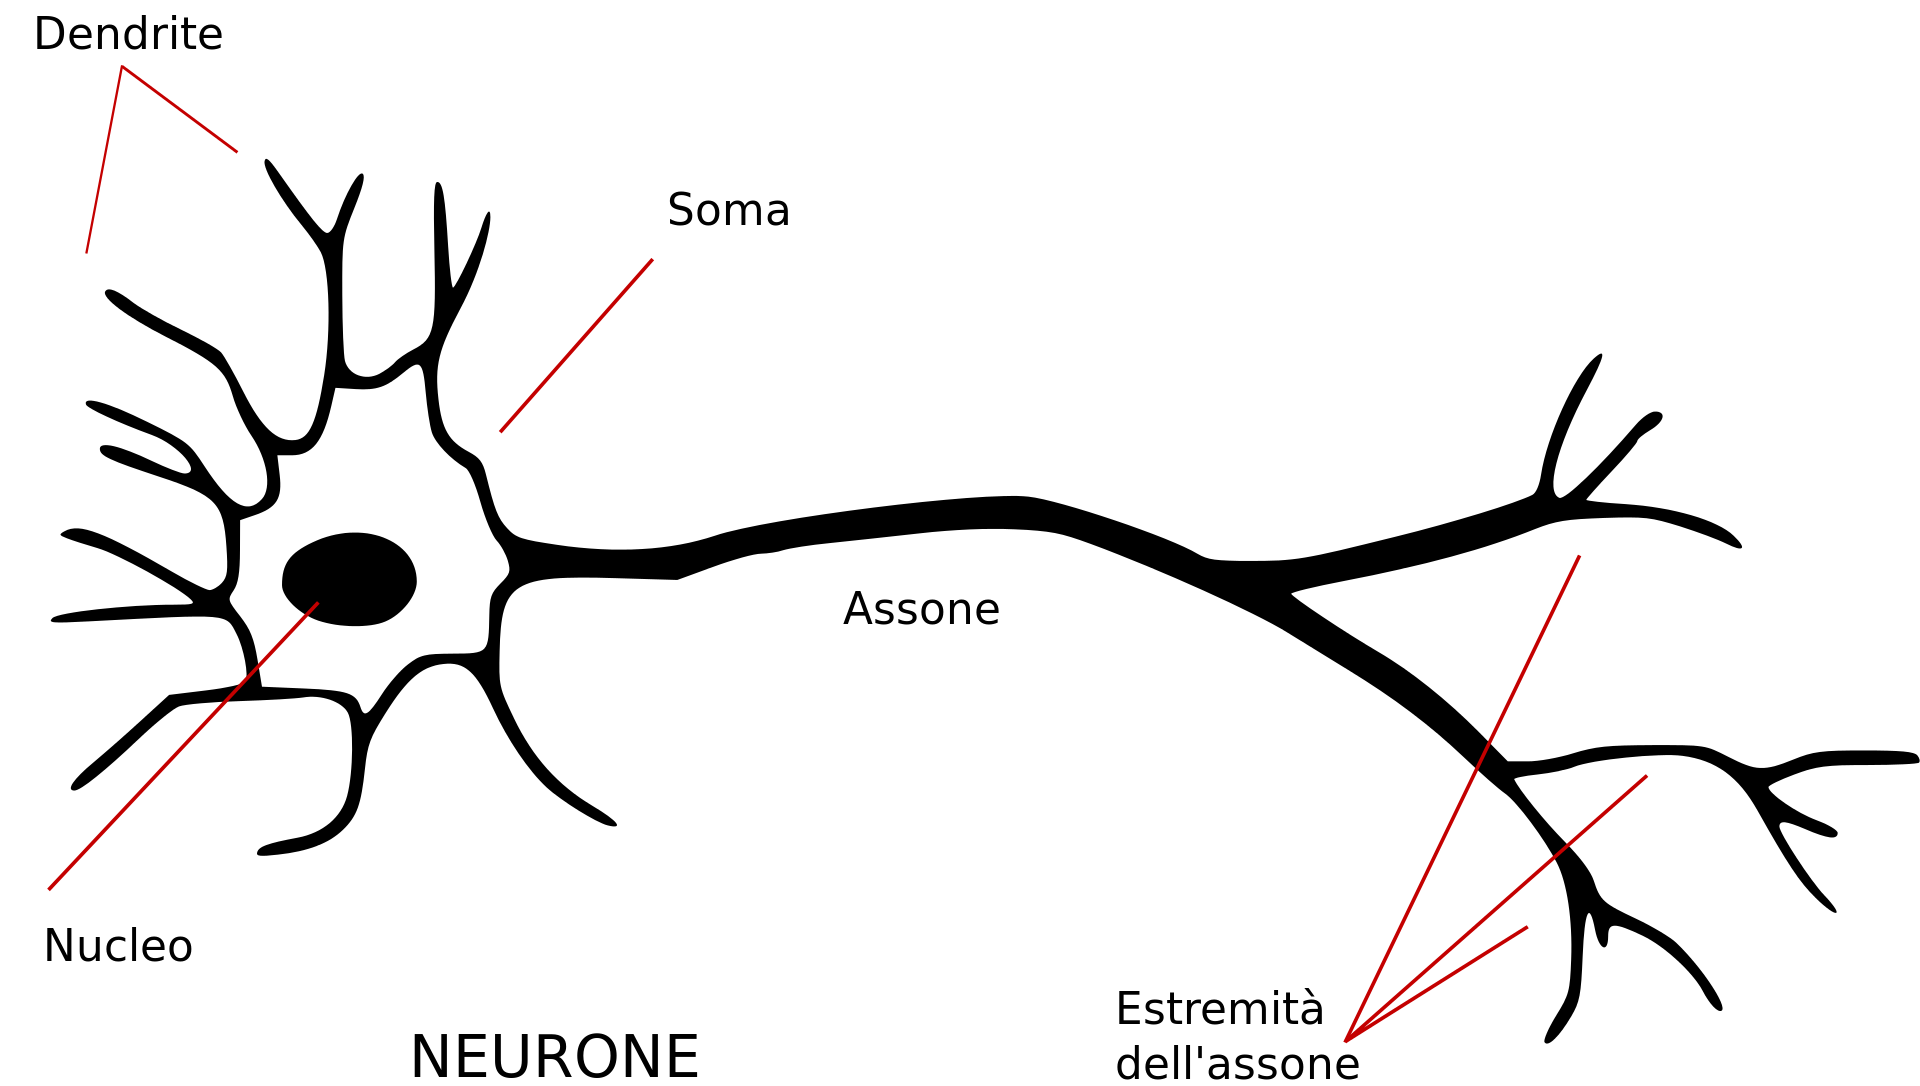
\includegraphics[width=0.75\textwidth]{Immagini/Generiche/Neurone.png}
    \caption{Esempio schematico di un neurone \cite{NEURONE_BIOLOGICO}.}
    \label{fig:esempioNeurone}
    %Figura 2.1: Esempio schematico di un neurone
\end{figure}

Infatti, un neurone, è un’unità che si occupa di compiere operazioni sulla base di
stimoli esterni e di propagare a sua volta lo stimolo.
Come si osserva dalla figura 2.1, un neurone, è composto da 3 parti principali:

\begin{itemize}
    \item  Il \textbf{soma}:  è il corpo cellulare. Si occupa di integrare tra loro i vari input
    corrispondenti agli stimoli esterni.

    \item L'\textbf{assone}:  l’unica linea di uscita del neurone che si dirama in migliaia di
    parti. Il soma restituisce un risultato che, nel caso in cui superi una certa
    soglia, il neurone si attiva e il cosiddetto "potenziale d’azione" (impulso
    elettrico) viene trasportato dall’assone. Al contrario, se il risultato non
    supera il valore di soglia il neurone rimane in uno stato di riposo.

    \item Il \textbf{dendrite}:  linea di entrata del neurone che riceve segnali in ingresso
    da altri assoni tramite le sinapsi, le quali a loro volta consentono la
    comunicazione con altri neuroni.
\end{itemize}

Il neurone è capace di ricevere segnali attraverso i propri dendriti, li elabora 
nel soma e successivamente trasmette il segnale, tramite l’assone, al neurone 
successivo. L’assone non è direttamente collegato ai dendriti di altri neuroni: 
il punto in cui il segnale viene trasmesso da una cellula ad un’altra è un 
piccolo spazio denominato “fessura sinaptica”. Quando un segnale è nei 
pressi di una sinapsi, questa rilascia un quantitativo di sostanze chimiche
chiamate “neurotrasmettitori”, i quali determinano la conduttività di una 
sinapsi, ovvero quanto la sinapsi attenua o enfatizza il segnale elettrico 
dall’assone. Nella trasmissione di un segnale, le correnti si possono sommare 
in spazio e tempo e se tale somma oltrepassa una certa soglia, un impulso di 
una certa entità e durata, denominato “potenziale d’azione”, è generato. Il 
segnale così prosegue per il prossimo assone, ricominciando il 
processo \cite{NEURONE_BIOLOGICO}.
% Le reti neurali si basano sulla simulazione di neuroni artificiali opportunamente 
% collegati, i quali ricevono in ingresso degli stimoli elaborandoli di conseguenza.